\documentclass[10pt,onecolumn,letterpaper]{article}

\usepackage{cvpr}
\usepackage{times}
\usepackage{epsfig}
\usepackage{graphicx}
\usepackage{amsmath}
\usepackage{amssymb}
\usepackage{dsfont}
\usepackage{outlines}
\usepackage[left=3cm, right=3cm, top=2cm]{geometry}

\newtheorem{theorem}{Theorem}
\DeclareMathOperator*{\argmin}{argmin}
\graphicspath{{./images/}}

% Include other packages here, before hyperref.


% If you comment hyperref and then uncomment it, you should delete
% egpaper.aux before re-running latex.  (Or just hit 'q' on the first latex
% run, let it finish, and you should be clear).
\usepackage[breaklinks=true,bookmarks=false]{hyperref}

\cvprfinalcopy % *** Uncomment this line for the final submission

\def\cvprPaperID{****} % *** Enter the CVPR Paper ID here
\def\httilde{\mbox{\tt\raisebox{-.5ex}{\symbol{126}}}}

% Pages are numbered in submission mode, and unnumbered in camera-ready
%\ifcvprfinal\pagestyle{empty}\fi
\setcounter{page}{1}
\begin{document}
%%%%%%%%% TITLE
\title{False Discoveries occur Early on the Lasso Path}

\author{
   Ramzi MISSAOUI\\
{\tt\small ramzi.missaoui@polytechnique.edu}
% For a paper whose authors are all at the same institution,
% omit the following lines up until the closing ``}''.
% Additional authors and addresses can be added with ``\and'',
% just like the second author.
% To save space, use either the email address or home page, not both
\and
Soufiane MOUTEI\\
{\tt\small soufiane.moutei@polytechnique.edu}
}

\maketitle
%\thispagestyle{empty}

%%%%%%%%% ABSTRACT
\begin{abstract}
   This report is written in the context of the the course “Theoretical guidelines for high-dimensional data analysis”, under the supervision of Christophe Giraud.
The goal of this report is to present a detailed analysis of the article  "False Discoveries occur Early on the Lasso Path” (https://arxiv.org/abs/1511.01957),  written by Weijie Su, Malgorzata Bogdan and Emmanuel Candes in November 2015, the most recent version being dated September 2016. We will try to grasp the key points, discuss the main results then talk about some limitations of the Lasso model. 

We'll have a quick reminder about the regression problem and the Lasso Method. Then we will move on to talk about the Lasso path and variable selection and talk about the theorem and its hypotheses. After that, we’ll highlight the limitations of the lasso and the issues caused by this type of regulation.

We also provide an implementation and a numerical analysis in the attached notebook which can be found in the address \textbf{**(drive link)** }The aim was to reproduce some of the experiments of the paper to highlight and check the results of the authors.
\end{abstract}

%%%%%%%%% BODY TEXT
\tableofcontents


\section{Introduction}

Statisticians have been facing many challenges when dealing with modern datasets in different fields such as finance, genetics, imaging… which amount to dealing with linear system of equations with more unknown variables than equations, let alone the fact that the equations are often corrupted by noisy measurements. This is where the lasso model comes to the rescue when dealing with high dimensional data.
\newline

Let’s first have a look at the classical version of the problem. The data is usually represented by the observation couples $(x_i, Y_i)  \in \mathbb{R}^p \times \mathbb{R}, i = 1 .. n;$. The goal is to find a regression function relating the predictors $x_i$ and the response $Y_i$.
The regression problem is formulated as follows:
$$
Y_i = \sum_{j=1}^p \beta_j X_{i,j} + \epsilon_i, \forall i = 1...n
$$

where: 

\begin{itemize}
   \item $ \epsilon$ is a vector of n independent and identically distributed random variables corresponding to a noise term.
   \item $X \in \mathbb{R}^n \times \mathbb{R}^p $ is the predicor variable where the $j^{th}$ column $X_j$ corresponds to the n observations of the $j^{th}$ predictor. 
   \item  $\beta \in \mathbb{R}^p$ is the unknown vector of coefficients for the regression function to be estimated using the data.
\end{itemize}

Under this configuration, and assuming that X has a full column rank, $\beta$ is estimated using the ordinary least squares technique, which yields:
$$
\hat{\beta} = \argmin_{b \in \mathbb{R}^p} \lVert Y - Xb \rVert_2^2 = \left(X^TX\right)^{-1}X^TY
$$
Then assuming that $ \mathbb{E}\epsilon_i = 0$ and $cov(\epsilon_i, \epsilon_j) = \sigma^2 \mathds{1}_{i=j} $, the model is evaluated using the mean squared prediction error (MSPE) giving:
$$
MSPE(\hat{\beta}) = \mathbb{E}\left(\frac{1}{n} \lVert X\left(\beta - \hat{\beta}\right) \rVert^2_2 \right) = \frac{p}{n}\sigma^2
$$

We can see here that the ordinary least squares method works pretty well in the case where $p \ll n$. 

However, in high dimensional data, where this particular condition is usually not satisfied, we need to work on a new method to tackle this problem.\\


\subsection{How about having a sparse estimator $\beta$ ?}

A sparse estimator which leads to select the most important variables and estimate their coefficients appears to be a practical solution, thus bringing us back to the previous case.

To ensure this sparsity, one might think about penalizing the number of non zero coefficients of the estimator in the below fashion:
$$
\hat{\beta} = \argmin_{b \in \mathbb{R}^p} \left( \frac{1}{n}\lVert Y - Xb \rVert_2^2 + \lambda \lVert b \rVert_0 \right )
$$
Where $\lVert b \rVert_0 = \sum_{k=1}^p \mathds{1}_{b_k \neq 0}$, the number of  nonzero components. 

$\lambda$ is chosen in a way to regulate the amount of nonzero elements in $\beta$, small values increase sparsity and vice-versa.

The previous problem is equivalent to:

$$
\hat{\beta} = \argmin_{\beta \in \beta_0[k]} \left( \frac{1}{n}\lVert Y - Xb \rVert_2^2 \right )
$$

where $\beta_0[k] = \left\{\beta;  \lVert \beta \rVert_0 < k\right\}$ 
\newline


This is clearly a non convex problem, proceeding that way would require to evaluate the objective for all the k possible combinations of $\beta$ which includes $\left( ^n_k\right) $ cases $\forall k = 1..p$. As k is unknown, one would end up testing $2^p = \sum_{k=1}^p \left( ^n_k\right)$ cases which is not feasable given the big values p can take.
\newline


\textbf{Can we convexify this problem?}
The answer is yes! By considering the $l_1$ norm instead of the $l_0$ norm, we happen to exactly deal with the Lasso estimator, which is the topic of the next section.

\subsection{Lasso presentation }

In the context of high dimensional data, where the number of features p is greater than the number of observations n, Lasso (Least absolute shrinkage and selection operator) can replace the ordinary least squares method.

One of the important features of the Lasso, especially compared to other techniques such as Ridge regression, is that it automatically reduces the number of variables. Indeed, the Lasso produces models where a large number of the regression coefficients are estimated to be equal to zero, if not most, thereby selecting the important variables.
\newline


Here is the formulation of Lasso estimator:
$$
\hat{\beta} = \argmin_{b \in \mathbb{R}^p} \left( \frac{1}{n}\lVert Y - Xb \rVert_2^2 + \lambda \lVert b \rVert_1 \right )
$$

where $\lVert b \rVert_1 = \sum_{i=1}^p \vert b_i \vert$ and $\lVert x \rVert_2^2 = \sum_{i=1}^n x_i^2 $
\newline

The hyper parameter $\lambda$ controls the strength of the regulation. Let's have a look at the extreme cases:
\begin{itemize}
   \item $\lambda = 0 \Rightarrow$ ordinary linear regression if $ p \leq n$.
   \item $\lambda = +\infty \Rightarrow$ All the coefficients of $\beta$ are zero. 
   \item The increase of $\lambda$ induces the decrease of some coefficients from $\hat{\beta}$ ending in the previous case scenario when it's big enough.
\end{itemize}

The previous lasso estimator can be reformulated as follows:
$$
\hat{\beta}(t) = \argmin_{b \in \mathbb{R}^p, \lVert b \rVert_1 \leq t} \lVert Y - Xb \rVert_2^2 
$$
\newline
In particular, this allows us to visualize in figure \ref{fig:lasso}, in 2 dimensions, the case where Lasso cancels one component ($\beta 1$), thus eliminates the predicor $x_1$, and \and shrinks the other ($\beta 2$) . 
\newline

The ellipses represent the counter lines for the function: $\beta \mapsto \lVert Y - X\beta \rVert_2^2 $. The left green square is nothing but the area where $\vert \beta_1 \vert + \vert \beta_2 \vert \leq t$ for a fixed $t$. We can observe that the lasso constraint has corners. Those pointy edges increase the chance of having a sparse solution.
\newline

The green circular area illustrates the case where we use the $\mathcal{L}_2$ norm, which corresponds to the Ridge regression problem.
The intersection between the counter lines and the green area gives the solutions of our optimization problem.  

\begin{figure}[!htbp]
   \begin{center}
	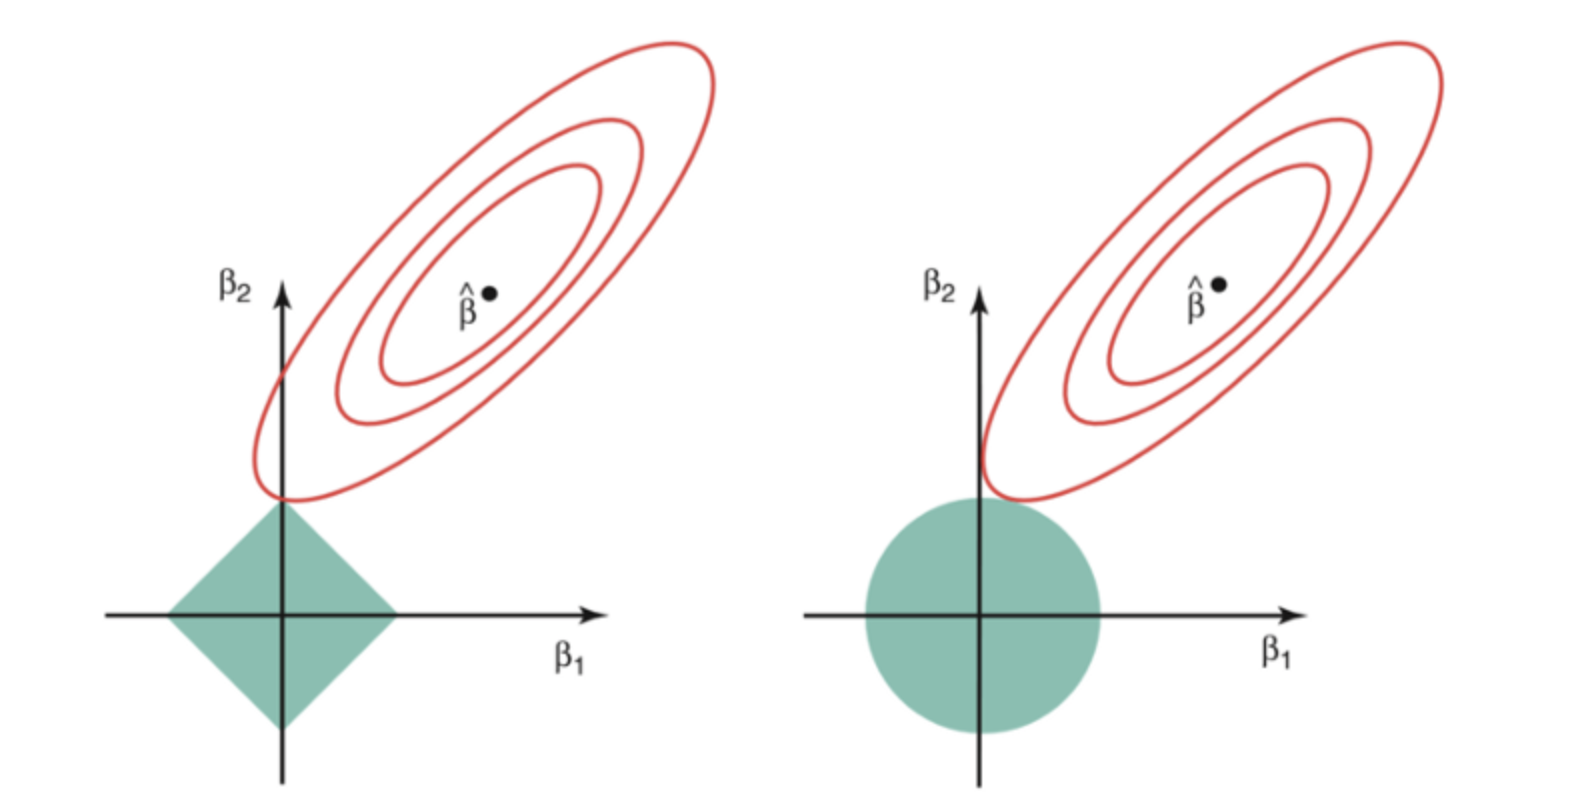
\includegraphics[width=0.7\linewidth]{lasso2d}
   \caption{Lasso in 2D}
   \label{fig:lasso}
   \end{center}
\end{figure}


\section{The model hypothesis and main results}

\subsection{Model Hypothesis }

\subsubsection{Working conditions}

We remind you that the paper put as in the design where $X \in \mathbb{R}^{n \times p}$, $ \beta \in \mathbb{R}^p$, and the errors $\epsilon \in \mathbb{R}^n$ 
In addition to that, the matrix \textbf{$\mathcal{X}$} has $i.i.d~\mathcal{N}(0,\frac{1}{n})$ elements, ensuring the normalization of the columns. As to the errors, $\epsilon_i$ are $i.i.d~\mathcal{N}(0,\sigma^2)$, where $\sigma$ is arbitrary choisen, yet fixed. The authors of the paper make the assumption that $\sigma$ can be zero, which corresponds to noiseless observation.


\subsubsection{Linear sparsity}
The article makes the assumption that the coefficients $\beta_1 ... \beta_p $ are independent copies of a random variable $\pi$ such that: $\mathbb{E}\pi < \infty $ and $\forall \epsilon \in \left[0,1\right], \mathbb{P}(\pi \neq 0) = \epsilon$

The article adds more limiting conditions when dealing with a high dimensional problem by setting:\\
 $\frac{p}{n} \to  \delta > 0; ~ p,n \to \infty$

In addition to these assumptions, the authors add a condition on the degree of sparsity. In fact, as cited in the paper, the expected number of nonzero regression coefficients is linear in p and equal to $\epsilon.p$ for $\epsilon > 0$. Therefore, this model is opposed to asymptotic discussions. For instance, in large dimension problems the proportion of non-zero coefficients tends towards zero, which is not the case here.

\subsubsection{Gaussian Designs}

The authors claim that the gaussian designs of the matrix $\mathcal{X}$ with independent columns are assumed to work in favor for model selection thanks to the low correlations between the features which the lasso takes advantage of.


Let us now turn to the main result of the article.


\subsection{Paper Stipulation }

This paper shows that, in a regime of linear sparsity and under the regression framework, the lasso does not perform as expected, which consists in, to cite the paper, finding “the important variables with few errors”. The authors show that it’s impossible to increase the True Positive Proportion (TPP)  \footnote{\label{tpp}\textbf{TPP} is defined as the ratio between the number of true discoveries and that of potential true discoveries to be made.},  which reflects finding the significant variables, without increasing the False Discovery Proportion (FDP) \footnote{\label{fdp}
\textbf{FDP} the ratio between the number of false discoveries and the total number of discoveries, along the Lasso path.} at the same time, which reflects the false discoveries . More formally, there is an asymptotic trade off between the False discovery Proportion and the True Positive Proportion.
\newline 

The authors claim that this result holds even in the case of the noiseless observation, $\sigma = 0$, which is a weak assumption.
\newline 

Let's recall the the lasso regression formulation:
$$
\hat{\beta} = \argmin_{b \in \mathbb{R}^p} \left( \frac{1}{n}\lVert Y - Xb \rVert_2^2 + \lambda \lVert b \rVert_1 \right )
$$

Then the FDP and the TPP are defined as follows:
$$
FDP = \frac{\vert \left\{ j: \hat{\beta}_j(\lambda) \neq 0, \beta_j = 0 \right\} \vert}{ max \left( \vert \left\{ j: \hat{\beta}_j(\lambda) \neq 0 \right\} \vert, 1 \right) }
$$

$$
TPP = \frac{\vert \left\{ j: \hat{\beta}_j(\lambda) \neq 0, \beta_j \neq 0 \right\} \vert}{ max \left( \vert \left\{ j: \hat{\beta}_j(\lambda) \neq 0 \right\} \vert, 1 \right) }
$$

The authors claim that this result holds even in the case of the noiseless observation, $\sigma = 0$, which is a weak assumption.
\newline


\textbf{Let's move on and have a look at the theorm.}


\subsection{Main Results}

\subsubsection{The Lasso Trade-off Diagram}


\begin{theorem}
Fix $\delta \in \left (0,\infty \right )$ and $ \epsilon \in \left (0,1 \right) $  and consider the function $ q^*(.) = q^*(.;\delta, \epsilon ) > 0 $; Then under the working hypothesis and for any arbitrary small constants $ \lambda_0 > 0$ and $\eta > 0$ then the event:
$$ \cap_{\lambda > \lambda_0} \left\{FDP(\lambda ) \geq q^* \left( TPP(\lambda)\right) - \eta \right\}
$$
 holds with a probabilty tending to one in both noisy and noiseless cases. 
\end{theorem}


 The function $q^*$ is called the boundary curve defined by:
 $$
q^*\left(u,\delta,\epsilon\right) = \frac{2(1-\epsilon)\Phi(-t^*(u))}{2(1-\epsilon)\Phi(-t^*(u)) + \epsilon u}
 $$

The fact that $q^*$ is strictly increasing illustrates the asymptotic trade-off between FDP and TPP. In fact, when TPP increases the lower bound of FDP gets higher, which leads to the increase of FDP with a probabilty tending to one. 
\newline

To better understand the behaviour of the function, you can find a display of some examples of it with different values of sparsity ($\epsilon$) and dimensionality ($\delta$) in figure ~\ref{fig:qfunction}.
\newline

An other interesting way to understand this trade-off, is by considering the FDP as a measure of the type I error, and 1 - TPP as a measure of type II error. Therefore, on the lasso path, both types of error rates cannot be simultaneously low. 
\newline

Figure \ref{fig:tradeoffdiagram} shows the Lasso trade-off diagram for two different cases. The boundary between the red and white area is assured by the function $q^*$. The red area is where both types of errors are small (ie high TPP and low FDP). This illustrates the paper's theorem as it says that the red region is not reachable on the Lasso path.
\newline

According to the last point of the theorem as cited in the paper, the boundary curve $q^*$ is tight, which means that if we take an other function $q$ such that there exists a point $u$ where $q(u) > q^*(u)$, q will will not satisfy the first two points of the theorem for some prior distribution $\Pi$ on the regressor coefficients.
\newline

This comes from the following fact: For any point $\left(u,q^∗(u) \right)$ on the curve, we can approach it by setting $\epsilon \prime \in (0,1)$ and setting the prior to be:

\begin{equation}
   \Pi = 
   \left\{
       \begin{aligned}
         &M,      &w.p.&\epsilon \epsilon \prime \\
         &M^{-1}, &w.p.&\epsilon(1-\epsilon \prime)\\
         &0,      &w.p.& 1 - \epsilon \\
       \end{aligned}
     \right.
 \end{equation}
\newline

And for any $u$ between 0 and 1 there is exists $\epsilon \prime > 0 $  such that

\begin{center}
$\lim\limits_{M \rightarrow +\infty} \lim\limits_{n,p \rightarrow +\infty}  (TPP(\lambda), FDP(\lambda)) \rightarrow  (u,q^*(u))$
\end{center}

\begin{figure}[!htbp]
   \begin{center}
	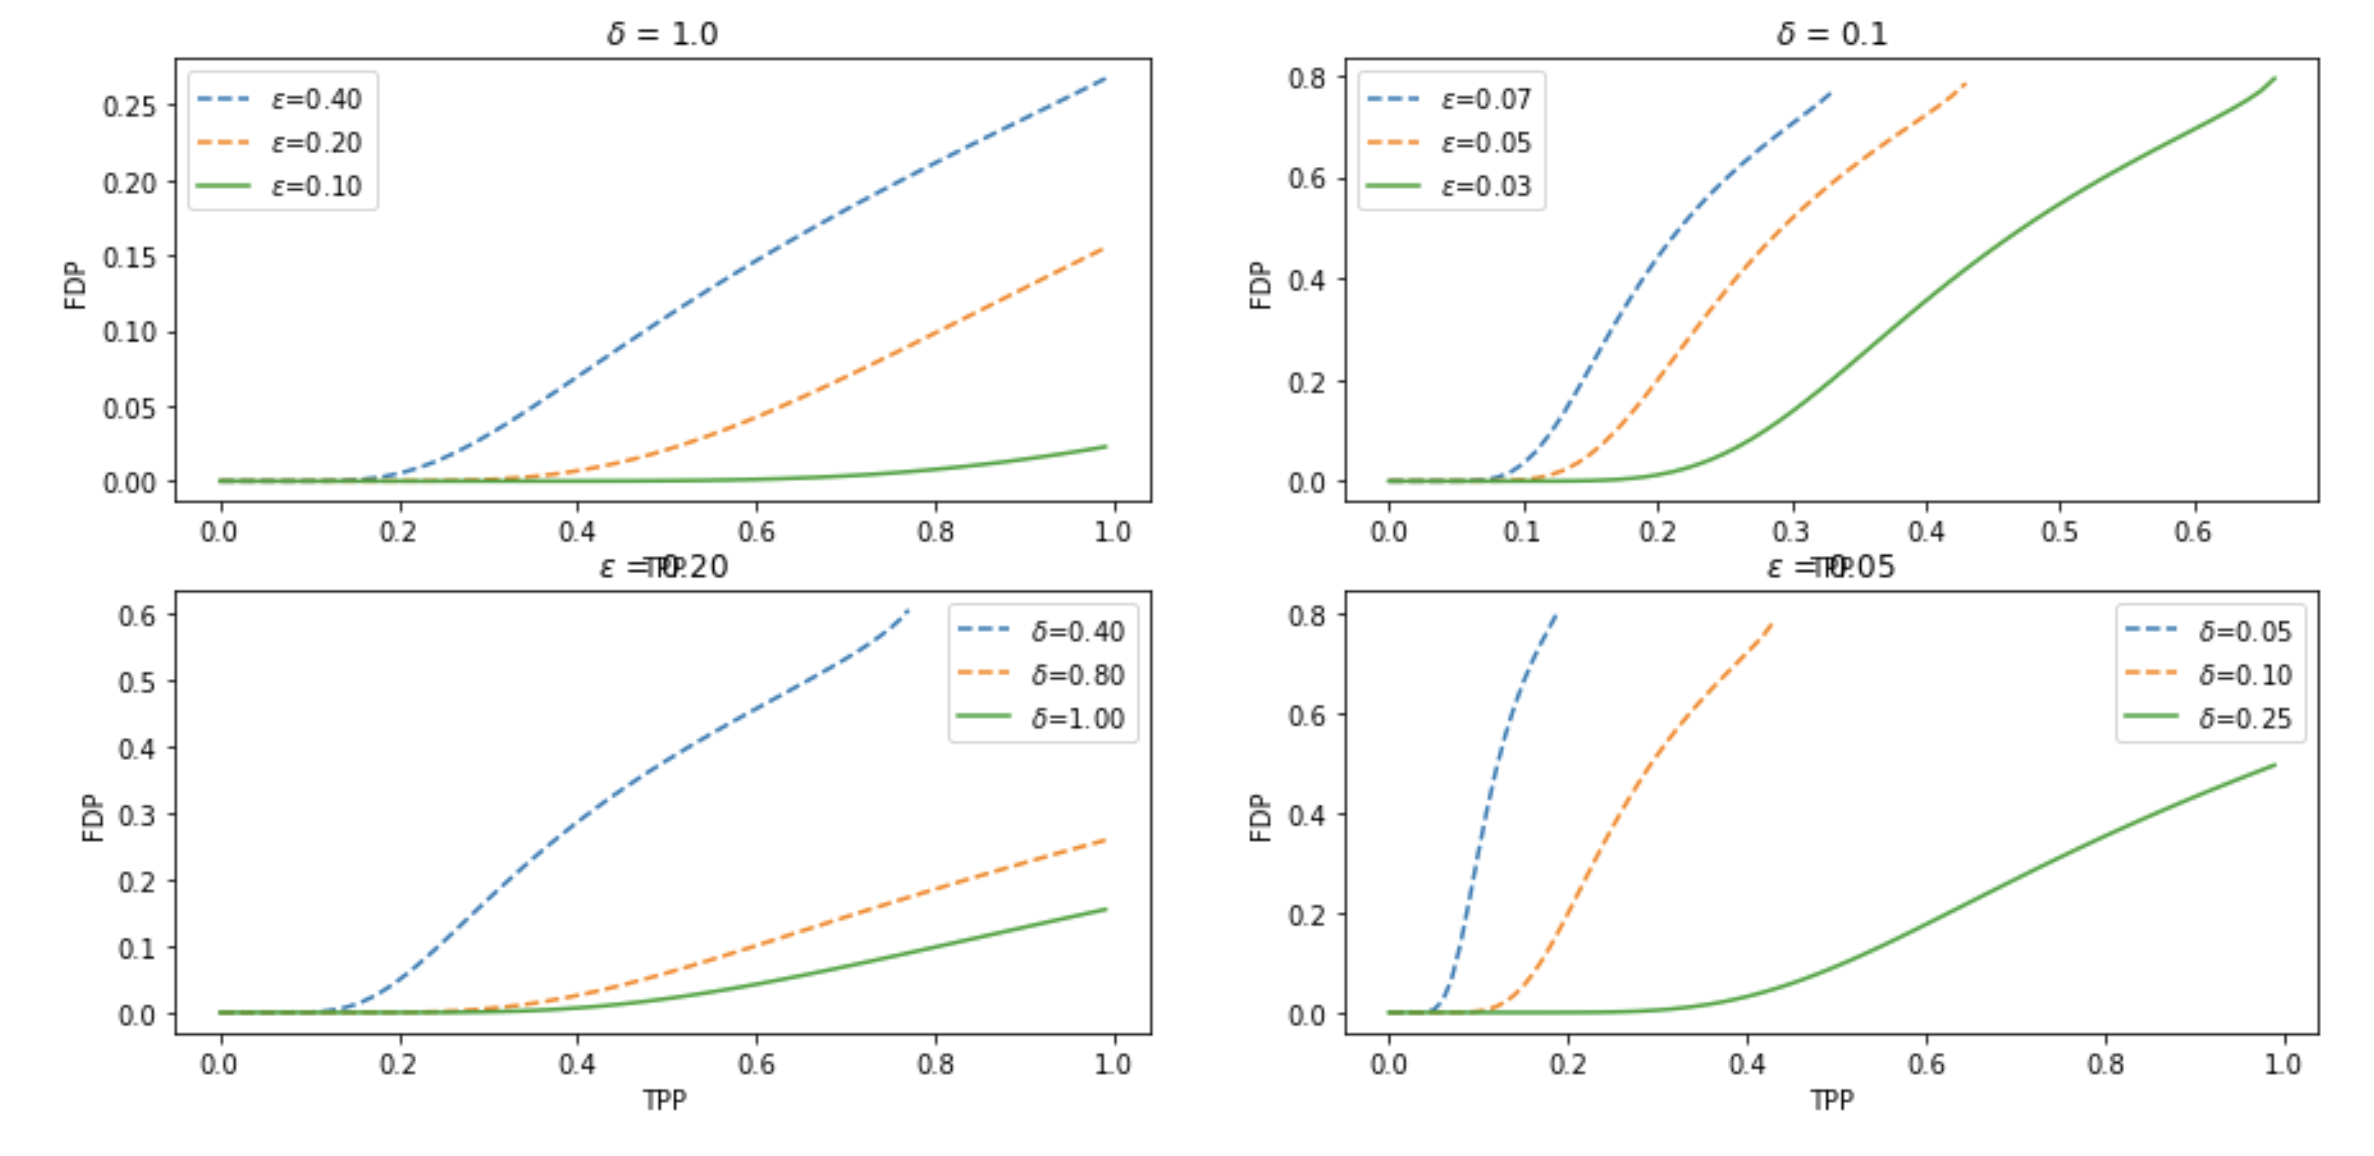
\includegraphics[width=0.9\linewidth]{qfunction}
   \caption{Top-left: $\delta = 1$; top-right: $\epsilon = 0.2$; bottom-left: $\delta = 0.1$; bottom-right: $\epsilon = 0.05$}
   \label{fig:qfunction}
   \end{center}
\end{figure}
%---
\begin{figure}[!htbp]
   \begin{center}
	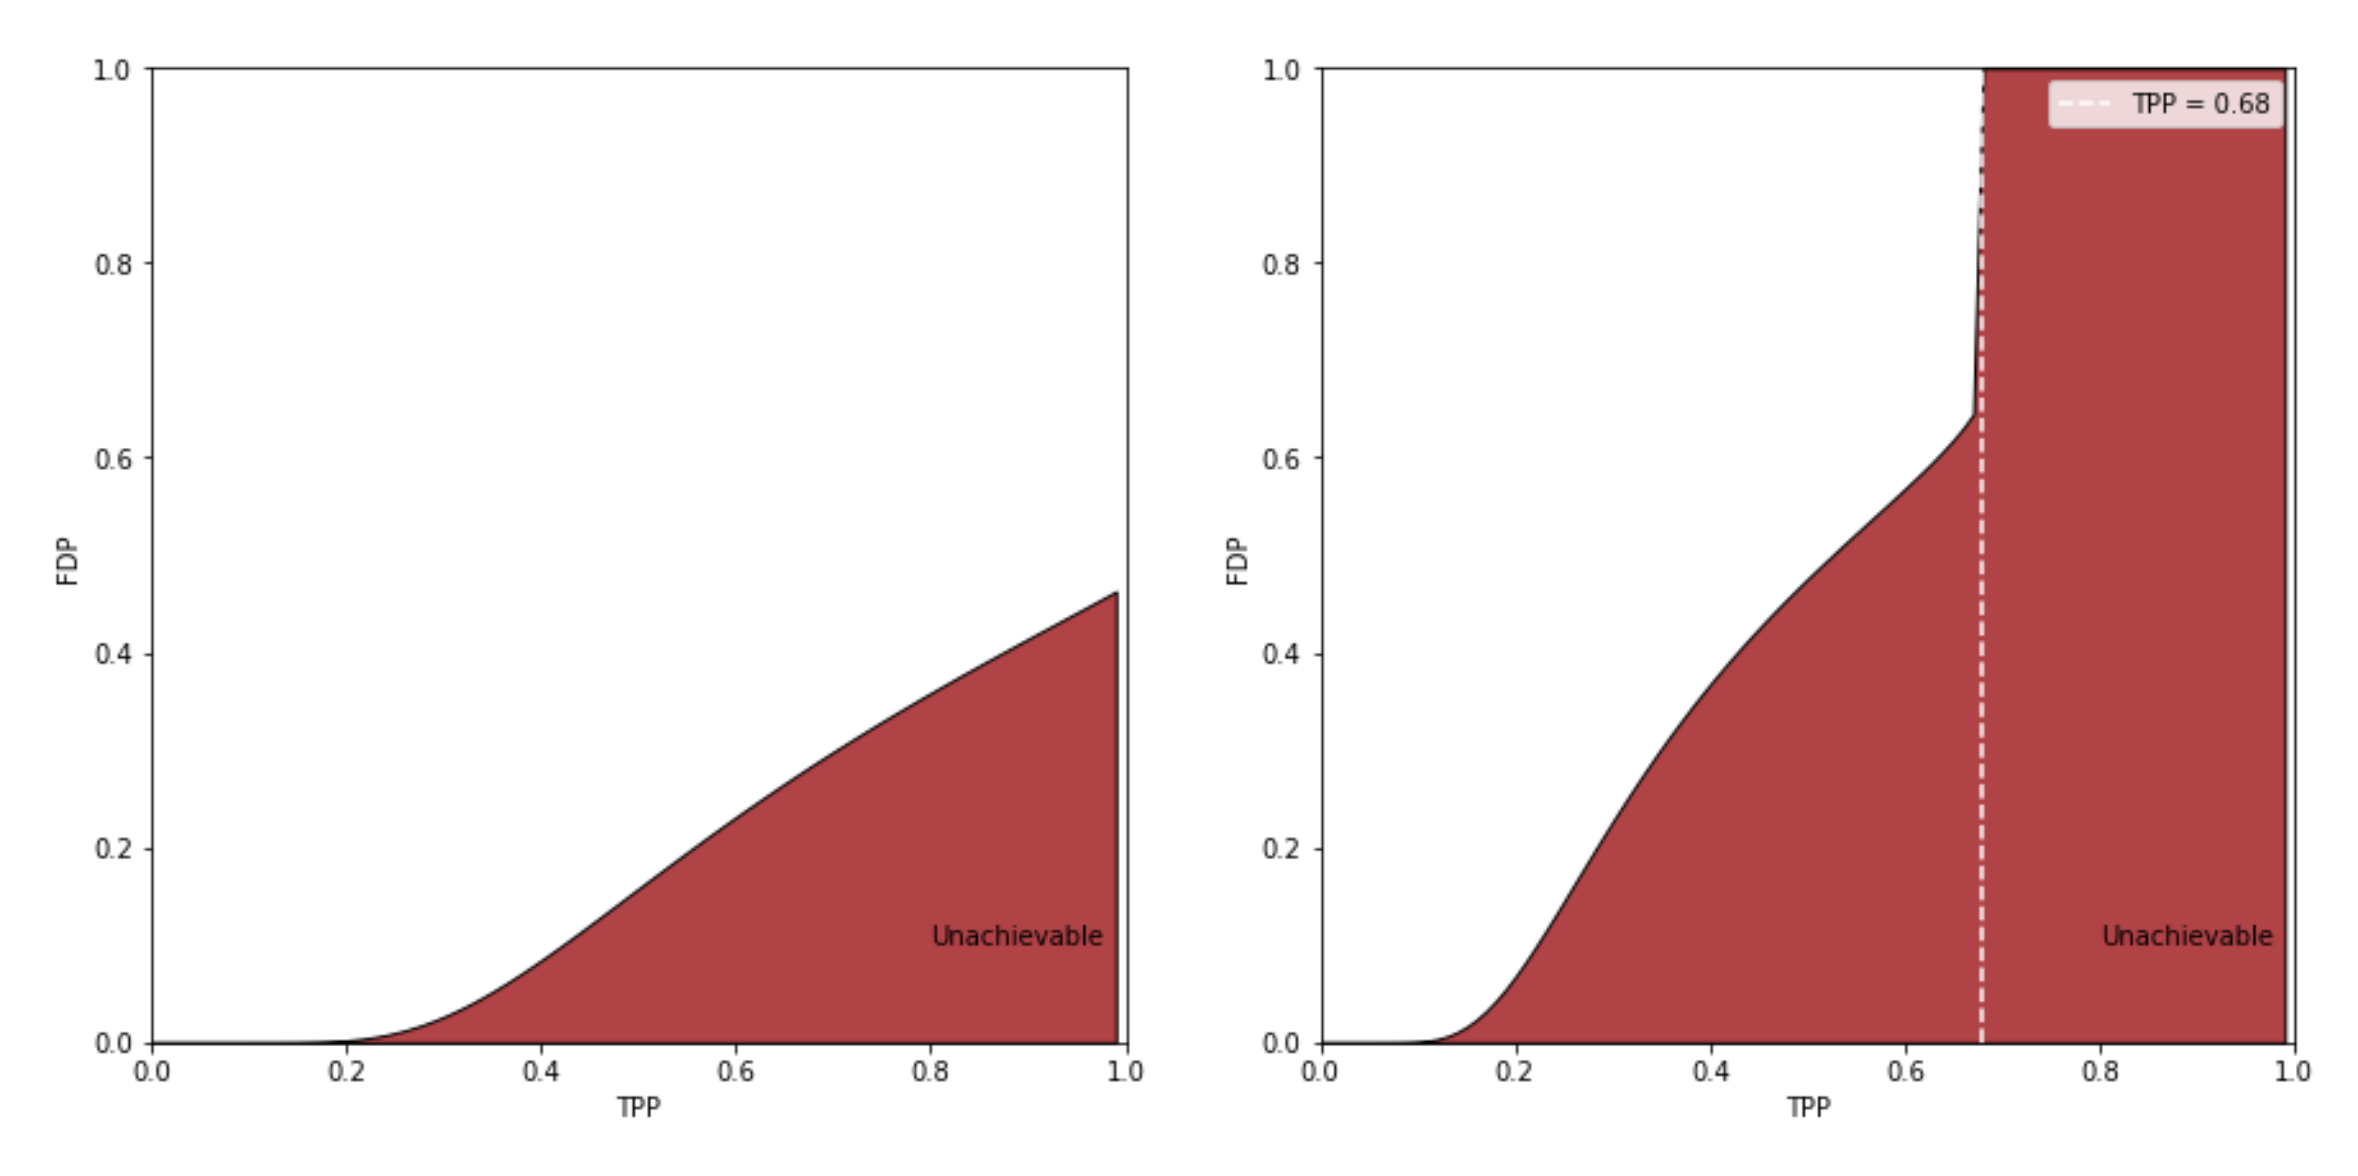
\includegraphics[width=0.9\linewidth]{tradeoffdiagram}
   \caption{\parbox[t]{8.5cm}{The Lasso trade-off diagram: left: $\delta = 0.5$ and $\epsilon = 0.15$; right:$\delta = 0.3$ and $\epsilon = 0.15$. The vertical truncation occurs at 0.6791). }}
   \label{fig:tradeoffdiagram}
   \end{center}
\end{figure}

\clearpage
\subsubsection{Lasso Shrinkage Noise}

We briefly mentioned earlier, when talking about the $\mathcal{L}_0$ regularization, that there are other methods to have a good model selection performance even under exponentional computations, thus sparing them from the difficulties in identifying variables in the model.
\newline 

Let's recall the $\mathcal{L}_0$-penalized maximum likelyhood estimate:

$$
\hat{\beta} = \argmin_{b \in \mathbb{R}^p} \left( \frac{1}{n}\lVert Y - Xb \rVert_2^2 + \lambda \lVert b \rVert_0 \right )
$$

Let's cite the second theorem from the paper:

\begin{theorem}
   Under our working hypothesis, take $\epsilon < \delta$ for identifiability, and consider the two- point prior:

   \begin{equation}
      \Pi = 
      \left\{
          \begin{aligned}
            &M,      &w.p. ~&\epsilon \\
            &0,      &w.p. ~& 1 - \epsilon \\
          \end{aligned}
        \right.
    \end{equation}
   Then we can find $\lambda(M)$ such that in probability, the discoveries of the $\mathcal{L}_0$ estimator obey:

   \begin{center}
      $\lim\limits_{M \rightarrow +\infty} \lim\limits_{n,p \rightarrow +\infty}  TPP(\lambda) = 1$
      $\lim\limits_{M \rightarrow +\infty} \lim\limits_{n,p \rightarrow +\infty}  FDP(\lambda) = 0$
      \end{center}


\end{theorem}

The theorem 2 highlights the absence of the asymptotic trade-off between TPP and FDP in the Ridge regression problem making it a better solution putting aside the computational limitations of the problem as it's non convex. 
\newline


Lasso limitations is mainly caused by the pseudo-noise introduced by the shrinkage. In fact, when the regularization factor is large, the lasso estimates get dwarfed. In other terms, if strong variables are selected, the penalty noise is inflated, and projecting it along the directions of some zero variables may actually eclipse the signal associated with the strong regression coefficients. It is for this reason that false discoveries enter the Lasso path.
\newline


Let's consider a reduced Lasso problem under the assumption that the true support $\mathcal{T}$ is a deterministic subset of size $\epsilon p$ in which each non-zero coefficient takes a value $M > 0$. We also assume $\delta > \epsilon$. To make things more challenging, we place ourselves in the noiseless case where $\sigma = 0$. 

$$
\hat{\beta}_{\mathcal{T}}(\lambda) = \argmin_{b_{\mathcal{T}} \in \mathbb{R}^{\epsilon p}}  \frac{1}{2}\lVert y - X_{\mathcal{T}}b_{\mathcal{T}} \rVert^2 + \lambda \lVert b_{\mathcal{T}} \rVert_1 
$$

The article then suggests to take $\lambda$ to have the same magnitude as $M$. The solution of the reduced lasso problem $\hat{\beta}_{\mathcal{T}}$ must verify the KKT conditions given by: 

$$
- \lambda \boldsymbol{1} < \mathcal{X}_{\mathcal{T}}^T(y - \mathcal{X}_{\mathcal{T}} \hat{\beta}_{\mathcal{T}}) \leq \lambda \boldsymbol{1}
$$

- When $\vert \mathcal{X}_{j}^T(y - \mathcal{X}_{\mathcal{T}} \hat{\beta}_{\mathcal{T}}) \vert \leq \lambda, \forall j \in \bar{\mathcal{T}} $, then completing $\hat{\beta}_{\mathcal{T}}(\lambda)$ whith zeros with give the solution to the full Lasso problem. 
\newline 

- If for $ j \in \bar{\mathcal{T}}$, $\vert \mathcal{X}_{j}^T(y - \mathcal{X}_{\mathcal{T}} \hat{\beta}_{\mathcal{T}}) \vert \leq \lambda $ then $X_j$ is selected by the incremental Lasso with design variables indexed by $\mathcal{T} \cup \{j\}$. 

Formally, this means that if we take $j \in \bar{\mathcal{T}}$ and define:

$$
\hat{\beta}_{\mathcal{T} \cup \{j\}}(\lambda) = \argmin_{b \in \mathbb{R}^{\epsilon p + 1}}  \frac{1}{2}\lVert y - X_{\mathcal{T} \cup \{j\}}b \rVert^2 + \lambda \lVert b \rVert_1 
$$

Then we have: $\hat{\beta}_j = 0$
\newline

All in All, two main points are worth mentionning:
\newline

First, if the full Lasso selects very few variables in $\bar{\mathcal{T}}$, then the value of the prediction $X\hat{\beta}$ will be very close to the one obtained in the reduced model.  

However, if the lasso selects only a small variable proportion from $\mathcal{T}$, hence a large proportion from $\bar{\mathcal{T}}$, then there would be a significant number of false discoveries. 

\section{Conclusion}

 

%-------------------------------------------------------------------------

{\small
\bibliographystyle{ieee}
\bibliography{egbib}
}

\end{document}
